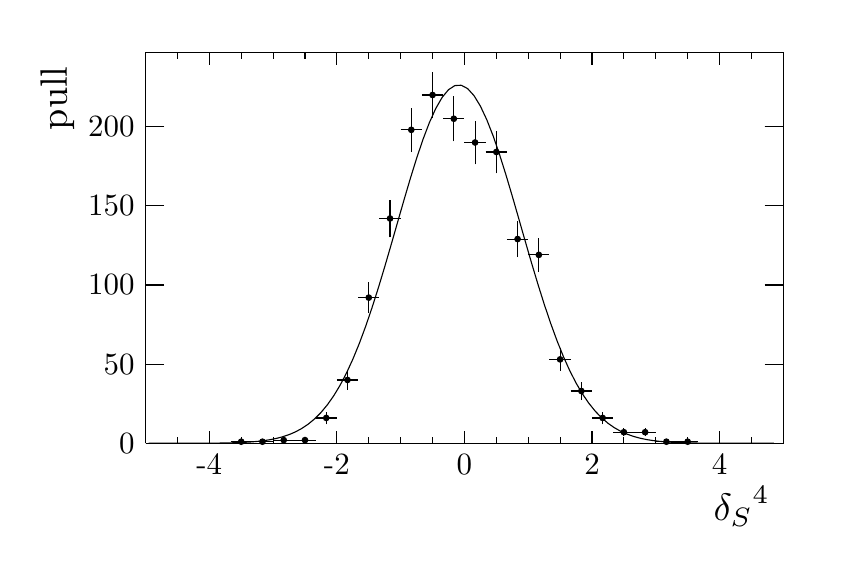
\begin{tikzpicture}
\pgfdeclareplotmark{cross} {
\pgfpathmoveto{\pgfpoint{-0.3\pgfplotmarksize}{\pgfplotmarksize}}
\pgfpathlineto{\pgfpoint{+0.3\pgfplotmarksize}{\pgfplotmarksize}}
\pgfpathlineto{\pgfpoint{+0.3\pgfplotmarksize}{0.3\pgfplotmarksize}}
\pgfpathlineto{\pgfpoint{+1\pgfplotmarksize}{0.3\pgfplotmarksize}}
\pgfpathlineto{\pgfpoint{+1\pgfplotmarksize}{-0.3\pgfplotmarksize}}
\pgfpathlineto{\pgfpoint{+0.3\pgfplotmarksize}{-0.3\pgfplotmarksize}}
\pgfpathlineto{\pgfpoint{+0.3\pgfplotmarksize}{-1.\pgfplotmarksize}}
\pgfpathlineto{\pgfpoint{-0.3\pgfplotmarksize}{-1.\pgfplotmarksize}}
\pgfpathlineto{\pgfpoint{-0.3\pgfplotmarksize}{-0.3\pgfplotmarksize}}
\pgfpathlineto{\pgfpoint{-1.\pgfplotmarksize}{-0.3\pgfplotmarksize}}
\pgfpathlineto{\pgfpoint{-1.\pgfplotmarksize}{0.3\pgfplotmarksize}}
\pgfpathlineto{\pgfpoint{-0.3\pgfplotmarksize}{0.3\pgfplotmarksize}}
\pgfpathclose
\pgfusepathqstroke
}
\pgfdeclareplotmark{cross*} {
\pgfpathmoveto{\pgfpoint{-0.3\pgfplotmarksize}{\pgfplotmarksize}}
\pgfpathlineto{\pgfpoint{+0.3\pgfplotmarksize}{\pgfplotmarksize}}
\pgfpathlineto{\pgfpoint{+0.3\pgfplotmarksize}{0.3\pgfplotmarksize}}
\pgfpathlineto{\pgfpoint{+1\pgfplotmarksize}{0.3\pgfplotmarksize}}
\pgfpathlineto{\pgfpoint{+1\pgfplotmarksize}{-0.3\pgfplotmarksize}}
\pgfpathlineto{\pgfpoint{+0.3\pgfplotmarksize}{-0.3\pgfplotmarksize}}
\pgfpathlineto{\pgfpoint{+0.3\pgfplotmarksize}{-1.\pgfplotmarksize}}
\pgfpathlineto{\pgfpoint{-0.3\pgfplotmarksize}{-1.\pgfplotmarksize}}
\pgfpathlineto{\pgfpoint{-0.3\pgfplotmarksize}{-0.3\pgfplotmarksize}}
\pgfpathlineto{\pgfpoint{-1.\pgfplotmarksize}{-0.3\pgfplotmarksize}}
\pgfpathlineto{\pgfpoint{-1.\pgfplotmarksize}{0.3\pgfplotmarksize}}
\pgfpathlineto{\pgfpoint{-0.3\pgfplotmarksize}{0.3\pgfplotmarksize}}
\pgfpathclose
\pgfusepathqfillstroke
}
\pgfdeclareplotmark{newstar} {
\pgfpathmoveto{\pgfqpoint{0pt}{\pgfplotmarksize}}
\pgfpathlineto{\pgfqpointpolar{44}{0.5\pgfplotmarksize}}
\pgfpathlineto{\pgfqpointpolar{18}{\pgfplotmarksize}}
\pgfpathlineto{\pgfqpointpolar{-20}{0.5\pgfplotmarksize}}
\pgfpathlineto{\pgfqpointpolar{-54}{\pgfplotmarksize}}
\pgfpathlineto{\pgfqpointpolar{-90}{0.5\pgfplotmarksize}}
\pgfpathlineto{\pgfqpointpolar{234}{\pgfplotmarksize}}
\pgfpathlineto{\pgfqpointpolar{198}{0.5\pgfplotmarksize}}
\pgfpathlineto{\pgfqpointpolar{162}{\pgfplotmarksize}}
\pgfpathlineto{\pgfqpointpolar{134}{0.5\pgfplotmarksize}}
\pgfpathclose
\pgfusepathqstroke
}
\pgfdeclareplotmark{newstar*} {
\pgfpathmoveto{\pgfqpoint{0pt}{\pgfplotmarksize}}
\pgfpathlineto{\pgfqpointpolar{44}{0.5\pgfplotmarksize}}
\pgfpathlineto{\pgfqpointpolar{18}{\pgfplotmarksize}}
\pgfpathlineto{\pgfqpointpolar{-20}{0.5\pgfplotmarksize}}
\pgfpathlineto{\pgfqpointpolar{-54}{\pgfplotmarksize}}
\pgfpathlineto{\pgfqpointpolar{-90}{0.5\pgfplotmarksize}}
\pgfpathlineto{\pgfqpointpolar{234}{\pgfplotmarksize}}
\pgfpathlineto{\pgfqpointpolar{198}{0.5\pgfplotmarksize}}
\pgfpathlineto{\pgfqpointpolar{162}{\pgfplotmarksize}}
\pgfpathlineto{\pgfqpointpolar{134}{0.5\pgfplotmarksize}}
\pgfpathclose
\pgfusepathqfillstroke
}
\definecolor{c}{rgb}{1,1,1};
\draw [color=c, fill=c] (0,0) rectangle (10,6.27517);
\draw [color=c, fill=c] (1.4,1.00403) rectangle (9.5,5.96141);
\definecolor{c}{rgb}{0,0,0};
\draw [c] (1.4,1.00403) -- (1.4,5.96141) -- (9.5,5.96141) -- (9.5,1.00403) -- (1.4,1.00403);
\draw [c] (2.615,1.00403) -- (2.615,1.02413);
\draw [c] (2.615,1.02413) -- (2.615,1.04424);
\draw [c] (2.48,1.02413) -- (2.615,1.02413);
\draw [c] (2.615,1.02413) -- (2.75,1.02413);
\foreach \P in {(2.615,1.02413)}{\draw[mark options={color=c,fill=c},mark size=2.402402pt,mark=*,mark size=1pt] plot coordinates {\P};}
\draw [c] (2.885,1.00403) -- (2.885,1.02413);
\draw [c] (2.885,1.02413) -- (2.885,1.04424);
\draw [c] (2.75,1.02413) -- (2.885,1.02413);
\draw [c] (2.885,1.02413) -- (3.02,1.02413);
\foreach \P in {(2.885,1.02413)}{\draw[mark options={color=c,fill=c},mark size=2.402402pt,mark=*,mark size=1pt] plot coordinates {\P};}
\draw [c] (3.155,1.0158) -- (3.155,1.04424);
\draw [c] (3.155,1.04424) -- (3.155,1.07267);
\draw [c] (3.02,1.04424) -- (3.155,1.04424);
\draw [c] (3.155,1.04424) -- (3.29,1.04424);
\foreach \P in {(3.155,1.04424)}{\draw[mark options={color=c,fill=c},mark size=2.402402pt,mark=*,mark size=1pt] plot coordinates {\P};}
\draw [c] (3.425,1.0158) -- (3.425,1.04424);
\draw [c] (3.425,1.04424) -- (3.425,1.07267);
\draw [c] (3.29,1.04424) -- (3.425,1.04424);
\draw [c] (3.425,1.04424) -- (3.56,1.04424);
\foreach \P in {(3.425,1.04424)}{\draw[mark options={color=c,fill=c},mark size=2.402402pt,mark=*,mark size=1pt] plot coordinates {\P};}
\draw [c] (3.695,1.24529) -- (3.695,1.32571);
\draw [c] (3.695,1.32571) -- (3.695,1.40613);
\draw [c] (3.56,1.32571) -- (3.695,1.32571);
\draw [c] (3.695,1.32571) -- (3.83,1.32571);
\foreach \P in {(3.695,1.32571)}{\draw[mark options={color=c,fill=c},mark size=2.402402pt,mark=*,mark size=1pt] plot coordinates {\P};}
\draw [c] (3.965,1.68107) -- (3.965,1.80823);
\draw [c] (3.965,1.80823) -- (3.965,1.93538);
\draw [c] (3.83,1.80823) -- (3.965,1.80823);
\draw [c] (3.965,1.80823) -- (4.1,1.80823);
\foreach \P in {(3.965,1.80823)}{\draw[mark options={color=c,fill=c},mark size=2.402402pt,mark=*,mark size=1pt] plot coordinates {\P};}
\draw [c] (4.235,2.66085) -- (4.235,2.85369);
\draw [c] (4.235,2.85369) -- (4.235,3.04653);
\draw [c] (4.1,2.85369) -- (4.235,2.85369);
\draw [c] (4.235,2.85369) -- (4.37,2.85369);
\foreach \P in {(4.235,2.85369)}{\draw[mark options={color=c,fill=c},mark size=2.402402pt,mark=*,mark size=1pt] plot coordinates {\P};}
\draw [c] (4.505,3.61936) -- (4.505,3.85894);
\draw [c] (4.505,3.85894) -- (4.505,4.09852);
\draw [c] (4.37,3.85894) -- (4.505,3.85894);
\draw [c] (4.505,3.85894) -- (4.64,3.85894);
\foreach \P in {(4.505,3.85894)}{\draw[mark options={color=c,fill=c},mark size=2.402402pt,mark=*,mark size=1pt] plot coordinates {\P};}
\draw [c] (4.775,4.70192) -- (4.775,4.98483);
\draw [c] (4.775,4.98483) -- (4.775,5.26773);
\draw [c] (4.64,4.98483) -- (4.775,4.98483);
\draw [c] (4.775,4.98483) -- (4.91,4.98483);
\foreach \P in {(4.775,4.98483)}{\draw[mark options={color=c,fill=c},mark size=2.402402pt,mark=*,mark size=1pt] plot coordinates {\P};}
\draw [c] (5.045,5.12893) -- (5.045,5.42714);
\draw [c] (5.045,5.42714) -- (5.045,5.72534);
\draw [c] (4.91,5.42714) -- (5.045,5.42714);
\draw [c] (5.045,5.42714) -- (5.18,5.42714);
\foreach \P in {(5.045,5.42714)}{\draw[mark options={color=c,fill=c},mark size=2.402402pt,mark=*,mark size=1pt] plot coordinates {\P};}
\draw [c] (5.315,4.8377) -- (5.315,5.12556);
\draw [c] (5.315,5.12556) -- (5.315,5.41342);
\draw [c] (5.18,5.12556) -- (5.315,5.12556);
\draw [c] (5.315,5.12556) -- (5.45,5.12556);
\foreach \P in {(5.315,5.12556)}{\draw[mark options={color=c,fill=c},mark size=2.402402pt,mark=*,mark size=1pt] plot coordinates {\P};}
\draw [c] (5.585,4.54686) -- (5.585,4.82399);
\draw [c] (5.585,4.82399) -- (5.585,5.10112);
\draw [c] (5.45,4.82399) -- (5.585,4.82399);
\draw [c] (5.585,4.82399) -- (5.72,4.82399);
\foreach \P in {(5.585,4.82399)}{\draw[mark options={color=c,fill=c},mark size=2.402402pt,mark=*,mark size=1pt] plot coordinates {\P};}
\draw [c] (5.855,4.43064) -- (5.855,4.70336);
\draw [c] (5.855,4.70336) -- (5.855,4.97607);
\draw [c] (5.72,4.70336) -- (5.855,4.70336);
\draw [c] (5.855,4.70336) -- (5.99,4.70336);
\foreach \P in {(5.855,4.70336)}{\draw[mark options={color=c,fill=c},mark size=2.402402pt,mark=*,mark size=1pt] plot coordinates {\P};}
\draw [c] (6.125,3.36923) -- (6.125,3.59758);
\draw [c] (6.125,3.59758) -- (6.125,3.82593);
\draw [c] (5.99,3.59758) -- (6.125,3.59758);
\draw [c] (6.125,3.59758) -- (6.26,3.59758);
\foreach \P in {(6.125,3.59758)}{\draw[mark options={color=c,fill=c},mark size=2.402402pt,mark=*,mark size=1pt] plot coordinates {\P};}
\draw [c] (6.395,3.17721) -- (6.395,3.39653);
\draw [c] (6.395,3.39653) -- (6.395,3.61585);
\draw [c] (6.26,3.39653) -- (6.395,3.39653);
\draw [c] (6.395,3.39653) -- (6.53,3.39653);
\foreach \P in {(6.395,3.39653)}{\draw[mark options={color=c,fill=c},mark size=2.402402pt,mark=*,mark size=1pt] plot coordinates {\P};}
\draw [c] (6.665,1.92323) -- (6.665,2.06959);
\draw [c] (6.665,2.06959) -- (6.665,2.21596);
\draw [c] (6.53,2.06959) -- (6.665,2.06959);
\draw [c] (6.665,2.06959) -- (6.8,2.06959);
\foreach \P in {(6.665,2.06959)}{\draw[mark options={color=c,fill=c},mark size=2.402402pt,mark=*,mark size=1pt] plot coordinates {\P};}
\draw [c] (6.935,1.552) -- (6.935,1.66749);
\draw [c] (6.935,1.66749) -- (6.935,1.78299);
\draw [c] (6.8,1.66749) -- (6.935,1.66749);
\draw [c] (6.935,1.66749) -- (7.07,1.66749);
\foreach \P in {(6.935,1.66749)}{\draw[mark options={color=c,fill=c},mark size=2.402402pt,mark=*,mark size=1pt] plot coordinates {\P};}
\draw [c] (7.205,1.24529) -- (7.205,1.32571);
\draw [c] (7.205,1.32571) -- (7.205,1.40613);
\draw [c] (7.07,1.32571) -- (7.205,1.32571);
\draw [c] (7.205,1.32571) -- (7.34,1.32571);
\foreach \P in {(7.205,1.32571)}{\draw[mark options={color=c,fill=c},mark size=2.402402pt,mark=*,mark size=1pt] plot coordinates {\P};}
\draw [c] (7.475,1.09157) -- (7.475,1.14476);
\draw [c] (7.475,1.14476) -- (7.475,1.19796);
\draw [c] (7.34,1.14476) -- (7.475,1.14476);
\draw [c] (7.475,1.14476) -- (7.61,1.14476);
\foreach \P in {(7.475,1.14476)}{\draw[mark options={color=c,fill=c},mark size=2.402402pt,mark=*,mark size=1pt] plot coordinates {\P};}
\draw [c] (7.745,1.09157) -- (7.745,1.14476);
\draw [c] (7.745,1.14476) -- (7.745,1.19796);
\draw [c] (7.61,1.14476) -- (7.745,1.14476);
\draw [c] (7.745,1.14476) -- (7.88,1.14476);
\foreach \P in {(7.745,1.14476)}{\draw[mark options={color=c,fill=c},mark size=2.402402pt,mark=*,mark size=1pt] plot coordinates {\P};}
\draw [c] (8.015,1.00403) -- (8.015,1.02413);
\draw [c] (8.015,1.02413) -- (8.015,1.04424);
\draw [c] (7.88,1.02413) -- (8.015,1.02413);
\draw [c] (8.015,1.02413) -- (8.15,1.02413);
\foreach \P in {(8.015,1.02413)}{\draw[mark options={color=c,fill=c},mark size=2.402402pt,mark=*,mark size=1pt] plot coordinates {\P};}
\draw [c] (8.285,1.00403) -- (8.285,1.02413);
\draw [c] (8.285,1.02413) -- (8.285,1.04424);
\draw [c] (8.15,1.02413) -- (8.285,1.02413);
\draw [c] (8.285,1.02413) -- (8.42,1.02413);
\foreach \P in {(8.285,1.02413)}{\draw[mark options={color=c,fill=c},mark size=2.402402pt,mark=*,mark size=1pt] plot coordinates {\P};}
\draw [c,line width=0.4] (1.4405,1.00403) -- (1.5215,1.00403) -- (1.6025,1.00403) -- (1.6835,1.00403) -- (1.7645,1.00403) -- (1.8455,1.00403) -- (1.9265,1.00403) -- (2.0075,1.00453) -- (2.0885,1.0048) -- (2.1695,1.00521) -- (2.2505,1.00581) --
 (2.3315,1.00669) -- (2.4125,1.00797) -- (2.4935,1.00979) -- (2.5745,1.01237) -- (2.6555,1.01597) -- (2.7365,1.02095) -- (2.8175,1.02776) -- (2.8985,1.03695) -- (2.9795,1.04923) -- (3.0605,1.06544) -- (3.1415,1.08658) -- (3.2225,1.11383) --
 (3.3035,1.14856) -- (3.3845,1.19227) -- (3.4655,1.24664) -- (3.5465,1.31344) -- (3.6275,1.39449) -- (3.7085,1.49161) -- (3.7895,1.60652) -- (3.8705,1.74071) -- (3.9515,1.89535) -- (4.0325,2.07116) -- (4.1135,2.26827) -- (4.1945,2.4861) --
 (4.2755,2.72326) -- (4.3565,2.97749) -- (4.4375,3.24558) -- (4.5185,3.52343) -- (4.5995,3.80607) -- (4.6805,4.08777) -- (4.7615,4.36225) -- (4.8425,4.62286) -- (4.9235,4.86286) -- (5.0045,5.07567) -- (5.0855,5.25523) -- (5.1665,5.39621) --
 (5.2475,5.49435) -- (5.3285,5.5466) -- (5.4095,5.55133);
\draw [c,line width=0.4] (5.4095,5.55133) -- (5.4905,5.50839) -- (5.5715,5.41913) -- (5.6525,5.28631) -- (5.7335,5.11399) -- (5.8145,4.90729) -- (5.8955,4.67216) -- (5.9765,4.41509) -- (6.0575,4.14282) -- (6.1385,3.86203) -- (6.2195,3.5791) --
 (6.3005,3.29988) -- (6.3815,3.02951) -- (6.4625,2.77225) -- (6.5435,2.53151) -- (6.6245,2.30972) -- (6.7055,2.10845) -- (6.7865,1.92842) -- (6.8675,1.76963) -- (6.9485,1.63148) -- (7.0295,1.51287) -- (7.1105,1.41236) -- (7.1915,1.32827) --
 (7.2725,1.2588) -- (7.3535,1.20212) -- (7.4345,1.15644) -- (7.5155,1.12006) -- (7.5965,1.09144) -- (7.6775,1.06919) -- (7.7585,1.05209) -- (7.8395,1.03911) -- (7.9205,1.02937) -- (8.0015,1.02214) -- (8.0825,1.01684) -- (8.1635,1.01299) --
 (8.2445,1.01023) -- (8.3255,1.00828) -- (8.4065,1.00691) -- (8.4875,1.00596) -- (8.5685,1.00531) -- (8.6495,1.00487) -- (8.7305,1.00458) -- (8.8115,1.00403) -- (8.8925,1.00403) -- (8.9735,1.00403) -- (9.0545,1.00403) -- (9.1355,1.00403) --
 (9.2165,1.00403) -- (9.2975,1.00403) -- (9.3785,1.00403);
\draw [c,line width=0.4] (9.3785,1.00403) -- (9.4595,1.00403);
\draw [c,line width=0.4] (1.4,1.00403) -- (9.5,1.00403);
\draw [anchor= east] (9.5,0.200805) node[scale=1.37879, rotate=0]{${\delta_\text{S}}^4$};
\draw [c,line width=0.4] (2.21,1.15651) -- (2.21,1.00403);
\draw [c,line width=0.4] (2.615,1.08027) -- (2.615,1.00403);
\draw [c,line width=0.4] (3.02,1.08027) -- (3.02,1.00403);
\draw [c,line width=0.4] (3.425,1.08027) -- (3.425,1.00403);
\draw [c,line width=0.4] (3.83,1.15651) -- (3.83,1.00403);
\draw [c,line width=0.4] (4.235,1.08027) -- (4.235,1.00403);
\draw [c,line width=0.4] (4.64,1.08027) -- (4.64,1.00403);
\draw [c,line width=0.4] (5.045,1.08027) -- (5.045,1.00403);
\draw [c,line width=0.4] (5.45,1.15651) -- (5.45,1.00403);
\draw [c,line width=0.4] (5.855,1.08027) -- (5.855,1.00403);
\draw [c,line width=0.4] (6.26,1.08027) -- (6.26,1.00403);
\draw [c,line width=0.4] (6.665,1.08027) -- (6.665,1.00403);
\draw [c,line width=0.4] (7.07,1.15651) -- (7.07,1.00403);
\draw [c,line width=0.4] (7.475,1.08027) -- (7.475,1.00403);
\draw [c,line width=0.4] (7.88,1.08027) -- (7.88,1.00403);
\draw [c,line width=0.4] (8.285,1.08027) -- (8.285,1.00403);
\draw [c,line width=0.4] (8.69,1.15651) -- (8.69,1.00403);
\draw [c,line width=0.4] (2.21,1.15651) -- (2.21,1.00403);
\draw [c,line width=0.4] (1.805,1.08027) -- (1.805,1.00403);
\draw [c,line width=0.4] (1.4,1.08027) -- (1.4,1.00403);
\draw [c,line width=0.4] (8.69,1.15651) -- (8.69,1.00403);
\draw [c,line width=0.4] (9.095,1.08027) -- (9.095,1.00403);
\draw [c,line width=0.4] (9.5,1.08027) -- (9.5,1.00403);
\draw [anchor=base] (2.21,0.602416) node[scale=1.11794, rotate=0]{-4};
\draw [anchor=base] (3.83,0.602416) node[scale=1.11794, rotate=0]{-2};
\draw [anchor=base] (5.45,0.602416) node[scale=1.11794, rotate=0]{0};
\draw [anchor=base] (7.07,0.602416) node[scale=1.11794, rotate=0]{2};
\draw [anchor=base] (8.69,0.602416) node[scale=1.11794, rotate=0]{4};
\draw [c,line width=0.4] (1.4,5.96141) -- (9.5,5.96141);
\draw [c,line width=0.4] (2.21,5.80892) -- (2.21,5.96141);
\draw [c,line width=0.4] (2.615,5.88517) -- (2.615,5.96141);
\draw [c,line width=0.4] (3.02,5.88517) -- (3.02,5.96141);
\draw [c,line width=0.4] (3.425,5.88517) -- (3.425,5.96141);
\draw [c,line width=0.4] (3.83,5.80892) -- (3.83,5.96141);
\draw [c,line width=0.4] (4.235,5.88517) -- (4.235,5.96141);
\draw [c,line width=0.4] (4.64,5.88517) -- (4.64,5.96141);
\draw [c,line width=0.4] (5.045,5.88517) -- (5.045,5.96141);
\draw [c,line width=0.4] (5.45,5.80892) -- (5.45,5.96141);
\draw [c,line width=0.4] (5.855,5.88517) -- (5.855,5.96141);
\draw [c,line width=0.4] (6.26,5.88517) -- (6.26,5.96141);
\draw [c,line width=0.4] (6.665,5.88517) -- (6.665,5.96141);
\draw [c,line width=0.4] (7.07,5.80892) -- (7.07,5.96141);
\draw [c,line width=0.4] (7.475,5.88517) -- (7.475,5.96141);
\draw [c,line width=0.4] (7.88,5.88517) -- (7.88,5.96141);
\draw [c,line width=0.4] (8.285,5.88517) -- (8.285,5.96141);
\draw [c,line width=0.4] (8.69,5.80892) -- (8.69,5.96141);
\draw [c,line width=0.4] (2.21,5.80892) -- (2.21,5.96141);
\draw [c,line width=0.4] (1.805,5.88517) -- (1.805,5.96141);
\draw [c,line width=0.4] (1.4,5.88517) -- (1.4,5.96141);
\draw [c,line width=0.4] (8.69,5.80892) -- (8.69,5.96141);
\draw [c,line width=0.4] (9.095,5.88517) -- (9.095,5.96141);
\draw [c,line width=0.4] (9.5,5.88517) -- (9.5,5.96141);
\draw [c,line width=0.4] (1.4,1.00403) -- (1.4,5.96141);
\draw [anchor= east] (0.28,5.96141) node[scale=1.37879, rotate=90]{pull};
\draw [c,line width=0.4] (1.637,1.00403) -- (1.4,1.00403);
\draw [c,line width=0.4] (1.637,2.00928) -- (1.4,2.00928);
\draw [c,line width=0.4] (1.637,3.01453) -- (1.4,3.01453);
\draw [c,line width=0.4] (1.637,4.01978) -- (1.4,4.01978);
\draw [c,line width=0.4] (1.637,5.02504) -- (1.4,5.02504);
\draw [c,line width=0.4] (1.637,5.02504) -- (1.4,5.02504);
\draw [anchor= east] (1.4,1.00403) node[scale=1.11794, rotate=0]{0};
\draw [anchor= east] (1.4,2.00928) node[scale=1.11794, rotate=0]{50};
\draw [anchor= east] (1.4,3.01453) node[scale=1.11794, rotate=0]{100};
\draw [anchor= east] (1.4,4.01978) node[scale=1.11794, rotate=0]{150};
\draw [anchor= east] (1.4,5.02504) node[scale=1.11794, rotate=0]{200};
\draw [c,line width=0.4] (9.5,1.00403) -- (9.5,5.96141);
\draw [c,line width=0.4] (9.263,1.00403) -- (9.5,1.00403);
\draw [c,line width=0.4] (9.263,2.00928) -- (9.5,2.00928);
\draw [c,line width=0.4] (9.263,3.01453) -- (9.5,3.01453);
\draw [c,line width=0.4] (9.263,4.01978) -- (9.5,4.01978);
\draw [c,line width=0.4] (9.263,5.02504) -- (9.5,5.02504);
\draw [c,line width=0.4] (9.263,5.02504) -- (9.5,5.02504);
\end{tikzpicture}
